\documentclass[12pt]{article}

\usepackage{amsmath, amssymb, amsthm, enumerate, graphicx}
\usepackage[usenames,dvipsnames]{color}
\usepackage{bm}
\usepackage[colorlinks=true,urlcolor=blue]{hyperref}
\usepackage{geometry}
\geometry{margin=1in}
\usepackage{float}
\usepackage{graphics}
\setlength{\marginparwidth}{2.15cm}
\usepackage{booktabs}
\usepackage{enumitem}
\usepackage{epsfig}
\usepackage{setspace}
\usepackage{parskip}
\usepackage[normalem]{ulem}
\usepackage{tikz}
\usetikzlibrary{positioning, arrows, automata}
\usepackage{pgfplots}
\usepackage[font=scriptsize]{subcaption}
\usepackage{float}
\usepackage[]{algorithm2e}
\usepackage{environ}
\usepackage{bbm}
\usepackage{graphicx}
\usepackage{titling}
\usepackage{url}
\usepackage{xcolor}
\usepackage{lipsum}
\usepackage{lastpage}
\usepackage[colorlinks=true,urlcolor=blue]{hyperref}
\usepackage{multicol}
\usepackage{tabularx}
\usepackage{comment}
\usepackage[utf8]{inputenc}
\usepackage{amssymb}
\usepackage{setspace}
\usepackage{marvosym}
\usepackage{wrapfig}
\usepackage{datetime}
\usepackage[many]{tcolorbox}
\usepackage{array}
\usepackage{multirow}
\usepackage{wasysym}
\usepackage{cancel}
\usepackage{xcolor} 
\usepackage{listings}
\usepackage{color}
\usepackage[thinlines]{easytable}
\usepackage{lastpage}

\newcommand{\R}{\mathbb{R}}
\newcommand{\blackcircle}{\tikz\draw[black,fill=black] (0,0) circle (1ex);}
\renewcommand{\circle}{\tikz\draw[black] (0,0) circle (1ex);}

\usetikzlibrary{positioning,calc}

\newtcolorbox[]{solution}[1][]{%
    breakable,
    enhanced,
    colback=white,
    %title=Solution,
    #1
}

\begin{document}
\section*{}
\begin{center}
  \centerline{\textsc{\LARGE  Homework 2 Template}}
\end{center}

Use this template to record your answers for Homework 2.  Add your answers using \LaTeX and then save your document as a PDF to upload to Gradescope.  You are required to use this template to submit your answers.  \textbf{You should not alter this template in any way} other than to insert your solutions.  You must submit all \pageref{LastPage} pages of this template to Gradescope.  Do not remove the instructions page(s).  Altering this template or including your solutions outside of the provided boxes can result in your assignment being graded incorrectly.  You may lose points if you do not follow these instructions.

Instructions to upload code have been provided in the handout.

\section*{Instructions for Specific Problem Types}

On this homework, you must fill in the blank for each problem; please make sure your final answer is fully included in the given space.  \textbf{Do not change the size of the box provided.}  For short answer questions you should \textbf{not} include your work in your solution.  Only provide an explanation or proof if specifically asked.  Otherwise, your assignment may not be graded correctly, and points may be deducted from your assignment.

\begin{quote}
\textbf{Fill in the blank:} What is the course number?

\begin{tcolorbox}[fit,height=1cm, width=4cm, blank, borderline={1pt}{-2pt},valign=center,nobeforeafter]
    \begin{center}\huge10-703\end{center}
    \end{tcolorbox}
\end{quote}

\newpage

\section*{Problem 0: Collaborators}
Enter your team's names and Andrew IDs in the boxes below.  If you do not do this, you may lose points on your assignment.

Name 1: \begin{tcolorbox}[fit,height=1cm, width=5cm, blank, borderline={1pt}{1pt},nobeforeafter]
    \begin{center}
    \vspace{3mm}
    \large{Arnav Goyal}
    \end{center}
\end{tcolorbox}
Andrew ID 1: \begin{tcolorbox}[fit,height=1cm, width=5cm, blank, borderline={1pt}{1pt},nobeforeafter]
    \begin{center}
    \vspace{3mm}
    \large{arnavgoy}
    \end{center}
\end{tcolorbox}
    \\
Name 2: \begin{tcolorbox}[fit,height=1cm, width=5cm, blank, borderline={1pt}{1pt},nobeforeafter]
    \begin{center}
    \vspace{3mm}
    \large{Vineeth Bhat}
    \end{center}
\end{tcolorbox}
Andrew ID 2: \begin{tcolorbox}[fit,height=1cm, width=5cm, blank, borderline={1pt}{1pt},nobeforeafter]
    \begin{center}
    \vspace{3mm}
    \large{vineethb}
    \end{center}
\end{tcolorbox} \\
Name 3: \begin{tcolorbox}[fit,height=1cm, width=5cm, blank, borderline={1pt}{1pt},nobeforeafter]
    \begin{center}
    \vspace{3mm}
    \large{Kushal Kejriwal}
    \end{center}
\end{tcolorbox}
Andrew ID 3: \begin{tcolorbox}[fit,height=1cm, width=5cm, blank, borderline={1pt}{1pt},nobeforeafter]
    \begin{center}
    \vspace{3mm}
    \large{kkejriwa}
    \end{center}
\end{tcolorbox} \\
\vspace{0.5cm}
\vspace{0.5cm}


\newpage
\section*{Problem 1: DQN (15 pts)}

\subsection*{1.1 DQN plot (15 pts)}
\begin{solution}[height=9cm]
\begin{figure}[H]
    \centering
    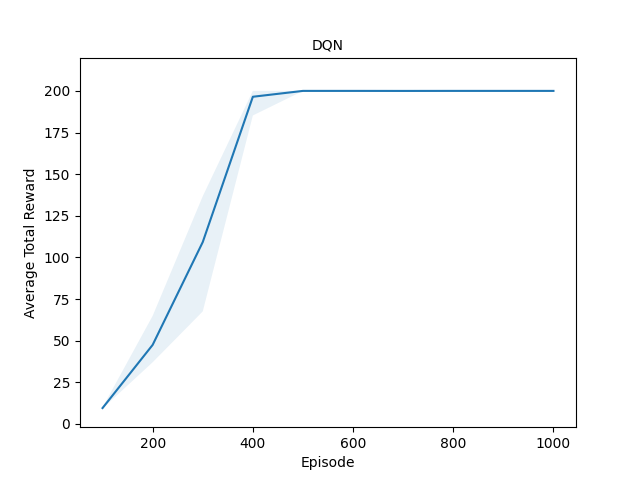
\includegraphics[width=0.68\textwidth]{graphs/DQN.png}
\end{figure}
\end{solution}


\newpage
\section*{Problem 2: Double DQN (21 pts)}

\subsection*{2.1: Double DQN plot (10 pts)}
\begin{solution}[height=9cm]
\begin{figure}[H]
    \centering
    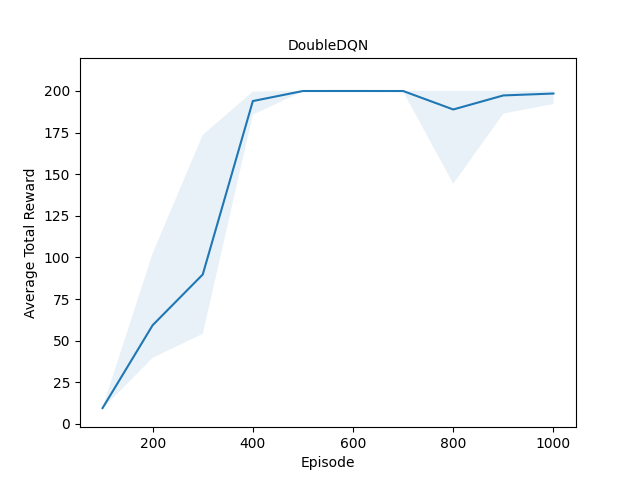
\includegraphics[width=0.68\textwidth]{graphs/DoubleDQN.png}
\end{figure}
\end{solution}

\subsection*{2.2 DQN vs. Policy Gradient Algorithms (5 pts)}
\begin{solution}[height=8cm]
DDQN reaches 200 in roughly 400 episodes, but REINFORCE with baseline and A2C with $N=100$ also saturate at 200 in HW1 and that too fairly fast ($\sim500$ episodes). DDQN \emph{only outperforms} plain REINFORCE and A2C with $N=1$ and $N=10$.

\emph{Sample efficiency.} Off-policy replay gives one minibatch update per environment step ($\sim200$ per episode) while PG takes one update per episode and discards the data. Caveat-this is per episode, not per gradient step, and DDQN also has a 10K burn-in.

\emph{Lower variance.} PG weights $\nabla_\theta\log\pi_\theta(a|s)$ by the whole-trajectory return $G_t$ from one correlated episode while TD targets use one transition plus a frozen target bootstrap with i.i.d. minibatches. So the wide bands across the 5 trials for REINFORCE and small-$N$ A2C against the narrow band here.

\small Also, with $|\mathcal{A}|=2$ and a deterministic best possible action, only the ordering of two $Q$-values matters, while an actor must separate its logits over many updates. Rewards are $+1$ everywhere, so all $Q>0$ and $\max_a Q$ overestimates, since the same network picks the action and reports its value. DDQN picks with the online net and evaluates with the target net, so the inflated action is no longer the one chosen, i.e, less bias therefore fewer flipped argmaxes.
\end{solution}

\subsection*{2.3 Pros and Cons of Policy gradient methods (6 pts)}
\begin{solution}[height=8cm]
\emph{A2C over DQN.} \textbf{(1)} Continuous or combinatorially large action spaces since DQN uses $\arg\max_a Q(s,a)$ at every step, which is intractable for $\mathcal{A}\subseteq\R^d$. \textbf{(2)} In some settings, we need a stochastic policy (e.g.m adverserial robustness) but a DQN policy is deterministic by construction ($\epsilon$-greedy is noise and not a stochastic representation). \textbf{3} DQN can have divergent behavior since frequency of target policy update is hand-crafted and you can have drift over replay buffer and current policy, while PG is just gradient descent and guarantees local optimum. \textbf{(4)} Cannot model action constraints in DQN.

\emph{DQN over A2C.} \textbf{(1)} DQN is better for small discrete $\mathcal{A}$ with expensive env. interaction since you store transitions in a replay buffer and can train over them again-and-again (\textbf{(2)} another interpretation: DQN is off-policy and therefore more sample efficient). \textbf{(3)} You can have high bias in DQN but not very high variance which is an issue as you grow your horizon in A2C, so DQN is better for long-horizon. \textbf{(4} learning the ordering of $Q$ is a weaker requirement than learning a policy distribution since you have denser rewards, and don't need to factor in stochasticity.
\end{solution}

\clearpage
\section*{Feedback}

\textbf{Feedback}: You can help the course staff improve the course for future semesters by providing feedback. You will receive a point of you provide actionable feedback. What was the most confusing part of this homework, and what would have made it less confusing?
\begin{solution}[height=4cm]
Function signatures for different functions would be really helpful in order to indicate typing of variables being passed through. This is double important in automated grading since a mismatch in data types that work for students' (accurate) implementation do not match the ones supplied by the automated grader leading to painful trial-and-error-s to get it right eventually. 
\end{solution}

\textbf{Collaboration}: Detail the work division amongst your group below.
\begin{solution}[height=4cm]
\begin{itemize}
    \item Arnav: 40\% implementation + 10\% report writing + theory. 
    \item Vineeth: 20\% implementation + 80\% report writing + theory.
    \item Kushal: Same division as Arnav.
\end{itemize}
\end{solution}

\noindent\textbf{Time Spent}: How many hours did you spend working on this assignment? Your answer will not affect your grade. Please average your answer over all the members of your team.
\begin{solution}[height=4cm]
\begin{table}[H]
    \centering
    \begin{tabular}{r|c}
        Alone & 2 hour \hspace{3em} %ANSWER HERE%
        \\ \hline
        With teammates & 4 hours \hspace{3em} %ANSWER HERE%
        \\ \hline
        With other classmates & 0.5 hours \hspace{3em} %ANSWER HERE%
        \\ \hline
        At office hours & 0 hours \hspace{3em} %ANSWER HERE%
        \\ \hline
    \end{tabular}
\end{table}
\end{solution}


\end{document}
